
%%%%%%%%%%%%%%%%%%%%%%%%%%%%%%%%%%%%%%%%%
% Landscape Poster
% LaTeX Template
%%%%%%%%%%%%%%%%%%%%%%%%%%%%%%%%%%%%%%%%%

\documentclass[a0,landscape]{a0poster}
\usepackage{multicol}
\usepackage{graphicx}
\usepackage{xcolor}
\usepackage{times}
\usepackage[utf8]{inputenc}
\usepackage{amsmath}
\usepackage{wrapfig}
\columnsep=100pt
\columnseprule=3pt

\begin{document}

%----------------------------------------------------------------------------------------
%	POSTER HEADER 
%----------------------------------------------------------------------------------------

\begin{minipage}[b]{0.8\linewidth}
\veryHuge \color{RoyalBlue} \textbf{From Hobby to Career: Exploring Professional eSports in Bangladesh} \color{Black}\\ % Title
\vspace{1cm}
\huge \textbf{MD Your Name (Your ID)} \par
\large Supervisor: Dr. Example Supervisor (Department of Example, University Name)
\end{minipage}
%
\begin{minipage}[b]{0.15\linewidth}

\includegraphics[width=12cm]{logo.png} % Logo
\end{minipage}

\vspace{1cm}

%----------------------------------------------------------------------------------------
% POSTER CONTENT
%----------------------------------------------------------------------------------------

\begin{multicols}{4}

%----------------------------------------------------------------------------------------
%	INTRODUCTION
%----------------------------------------------------------------------------------------

\section*{Introduction}
eSports has grown from a recreational activity into a professional industry. This study examines the evolution of eSports in Bangladesh, with a focus on financial prospects, societal challenges, and the inspiration for players transitioning into professionals.

%----------------------------------------------------------------------------------------
%	RESEARCH OBJECTIVES
%----------------------------------------------------------------------------------------

\section*{Research Objectives}
\begin{itemize}
    \item To assess the financial viability of eSports in Bangladesh.
    \item To identify the motivations and challenges of professional players.
    \item To analyze societal perceptions of eSports as a career.
\end{itemize}

%----------------------------------------------------------------------------------------
% METHODOLOGY
%----------------------------------------------------------------------------------------

\section*{Methodology}
The study used surveys and interviews to collect data from professional and aspiring eSports players. Snowball sampling was employed to ensure a wide participant pool. Data analysis was conducted using statistical and visualization tools.

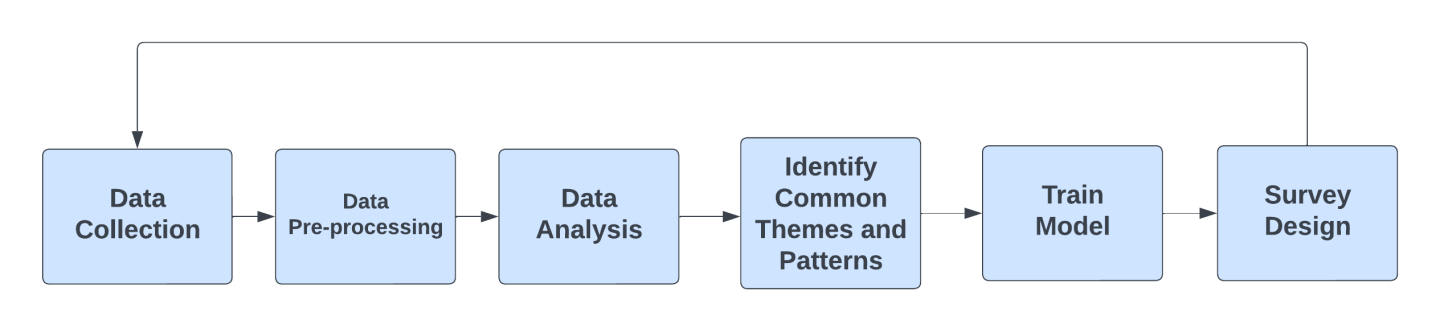
\includegraphics[width=\linewidth]{Workflow_1.png}
\captionof{figure}{\color{Green} Research Workflow}

%----------------------------------------------------------------------------------------
% FINDINGS
%----------------------------------------------------------------------------------------

\section*{Findings}

\subsection*{Income Distribution}
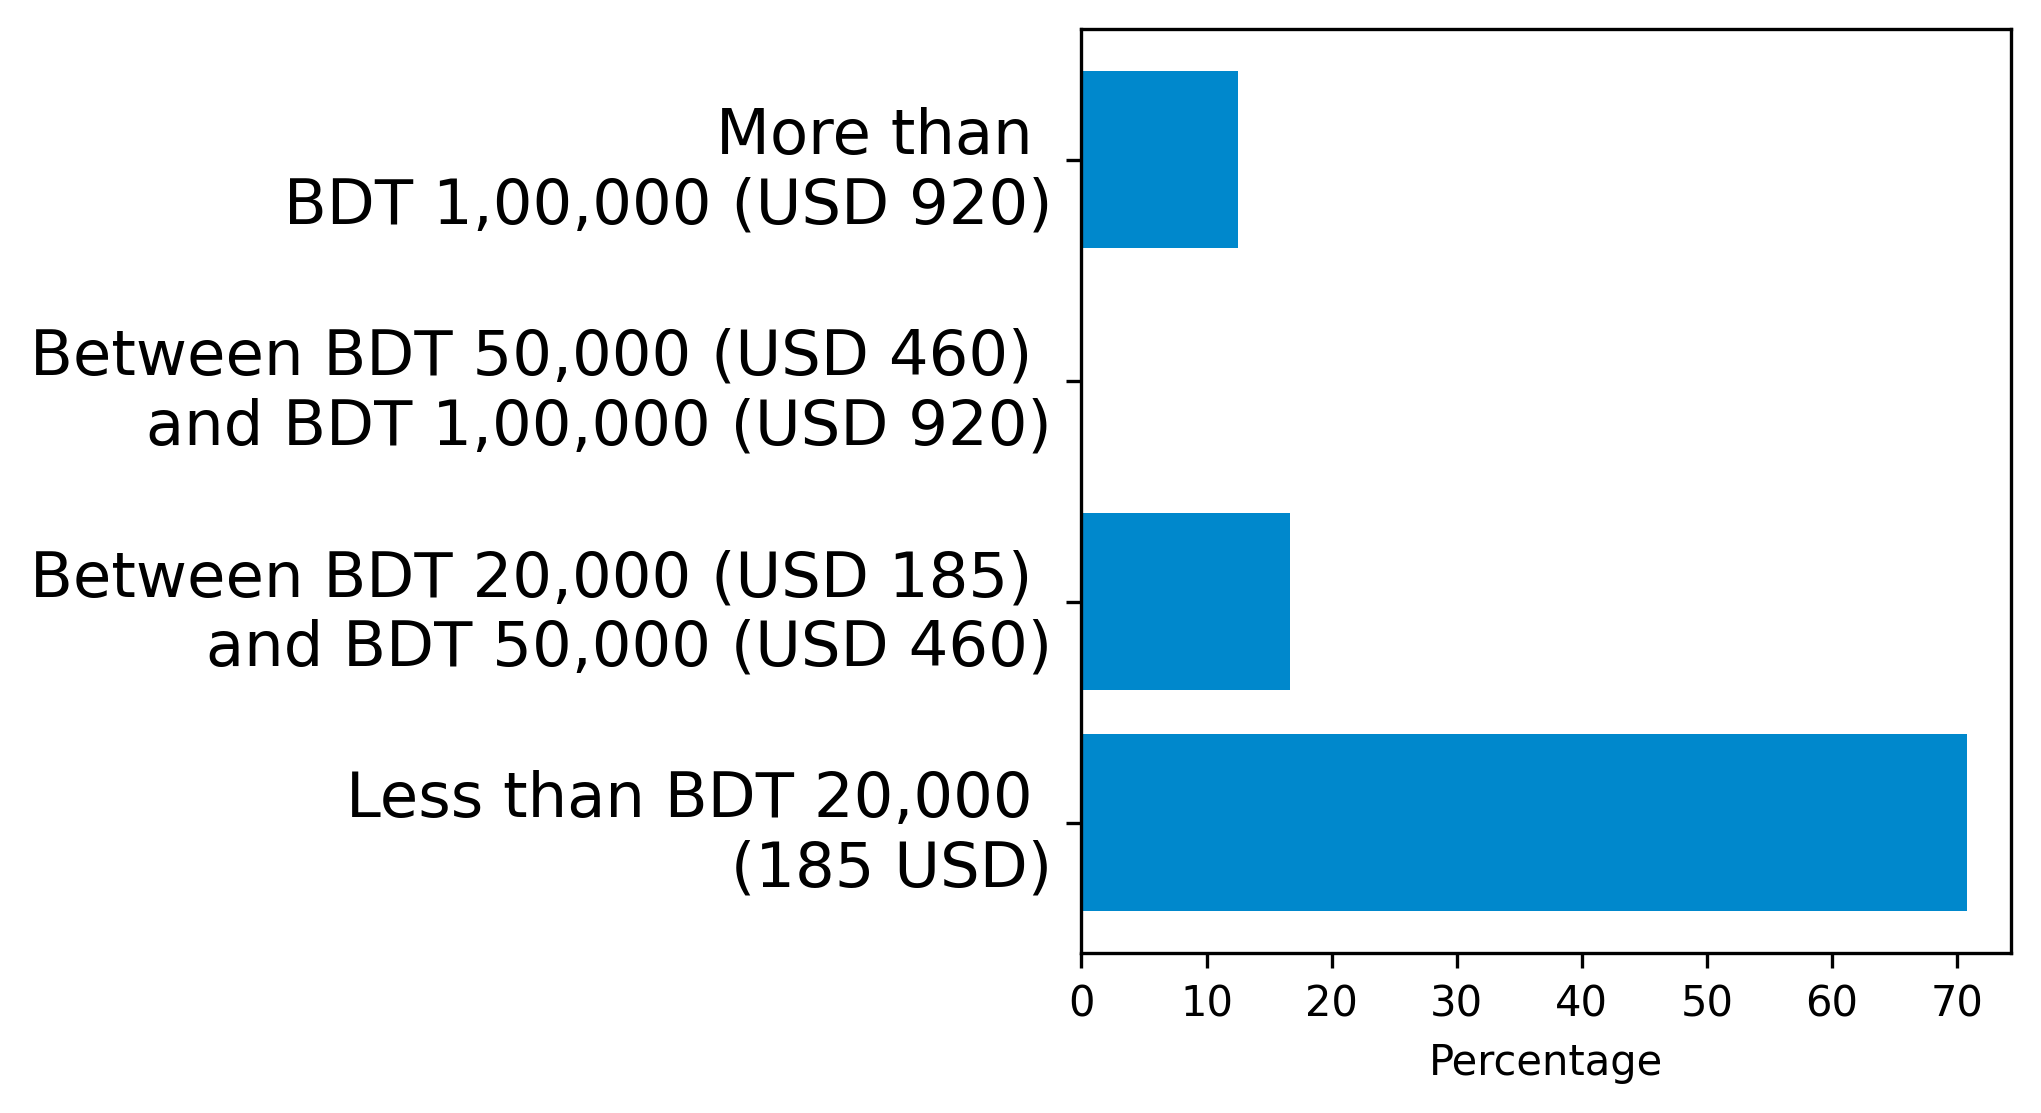
\includegraphics[width=\linewidth]{EA4.png}

\subsection*{Motivations}
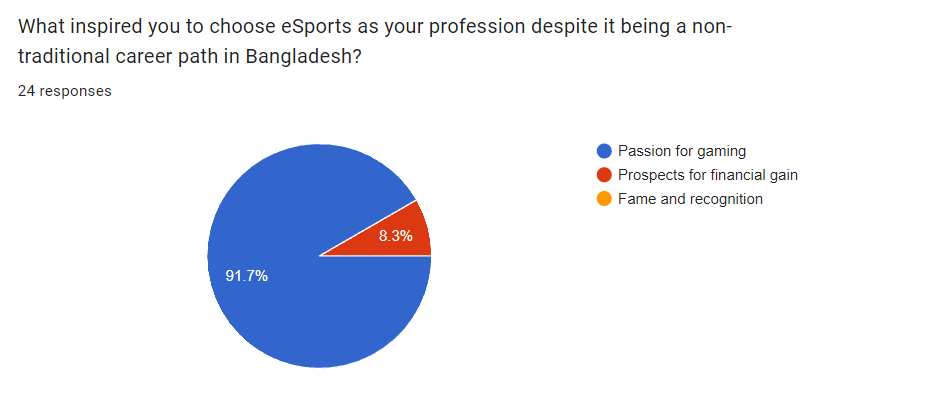
\includegraphics[width=\linewidth]{inspiration.png}

\subsection*{Challenges}
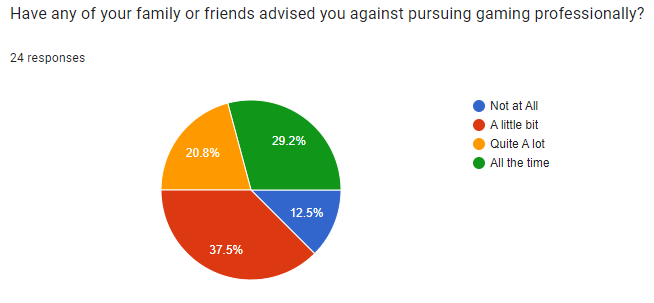
\includegraphics[width=\linewidth]{challenges.png}

%----------------------------------------------------------------------------------------
% FAMILY SUPPORT AND PERCEPTION
%----------------------------------------------------------------------------------------

\section*{Family Support and Perception}
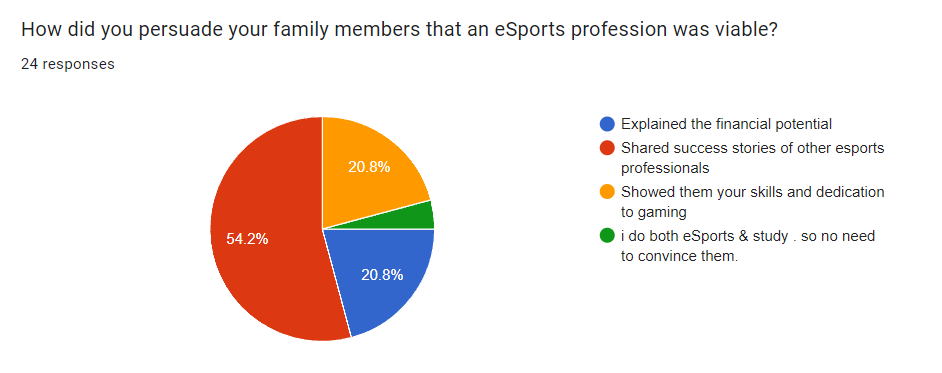
\includegraphics[width=\linewidth]{persuade your family.png}

%----------------------------------------------------------------------------------------
%	CONCLUSIONS
%----------------------------------------------------------------------------------------

\section*{Conclusion}
eSports in Bangladesh shows significant potential despite facing financial and societal hurdles. Passion for gaming remains a strong motivator for many players, underscoring the need for institutional support and broader acceptance of eSports as a viable career path.

%----------------------------------------------------------------------------------------
%	REFERENCES
%----------------------------------------------------------------------------------------

\section*{References}
\bibliographystyle{plain}
\bibliography{references}

\end{multicols}
\end{document}
